\documentclass{report}
\usepackage{graphicx}
\usepackage{float}
\usepackage[a4paper, top=20mm, bottom=20mm, left=25mm, right=25mm]{geometry}
\usepackage{subcaption}
\usepackage{titlesec}
\title{Visual Computing Assignment 2}

\author{Ebbe Wertz, Mathias Houwen}
\date{22 April 2025}

\begin{document}

\maketitle

\section{Decoding Gray Codes from Structured Light}
\label{sec:gray}

The images were acquired using the Structured Light method, in which a series of binary-encoded light patterns are projected onto a scene both vertically and horizontally. Each pixel is either illuminated or in shadow. As the width of the patterns decreases exponentially, the sequence of bright and dark values at each pixel forms a binary number, with each frame representing one bit. Given the reference patterns, these binary sequences follow the Gray code ordering.

To decode a frame, two images are used: one with the light pattern and one with its inverse. This dual-frame approach is crucial, as naive thresholding might misclassify regions that are always in shadow as dark, when in fact they should be considered invalid. To correctly classify each pixel, the difference between the normal and inverted images is calculated. If the difference exceeds a positive or negative threshold, the pixel is classified as either lit or dark, respectively. Pixels with differences near zero are marked as unreliable. Figure~\ref{fig:graycode} illustrates this classification process.

\begin{figure}[H]
    \centering
    \begin{subfigure}[b]{0.45\linewidth}
        \centering
        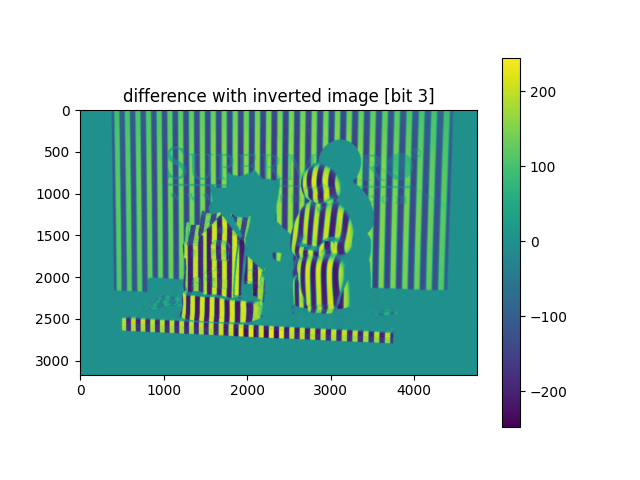
\includegraphics[height=50mm, keepaspectratio]{report_images/1_gray_codes/diff.png}
    \end{subfigure}
    \hfill
    \begin{subfigure}[b]{0.45\linewidth}
        \centering
        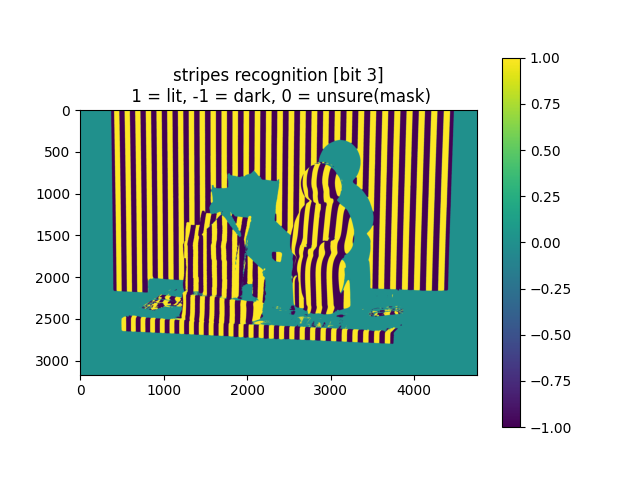
\includegraphics[height=50mm, keepaspectratio]{report_images/1_gray_codes/class.png}
    \end{subfigure}
    \caption{Lit or dark classification based on the difference image}
    \label{fig:graycode}
\end{figure}

The regions that remain in shadow throughout all frames are clearly visible as zero values in the right plot. This classification process is applied iteratively across all frames. A boolean mask is updated via bitwise OR operations, and the decoded values for both vertical and horizontal patterns are updated by setting the corresponding bit for each lit pixel. Finally, the binary values are decoded from Gray code into standard binary. This ensures the resulting values are consistent and sorted, assuming an ideal (non-perspective distorted) projection.

To visualize the decoded data, the values can be mapped to colors, generating false color images. These visualizations are shown in Figure~\ref{fig:graycodes_visualised}.

\begin{figure}[H]
    \centering
    \begin{subfigure}[b]{0.45\linewidth}
        \centering
        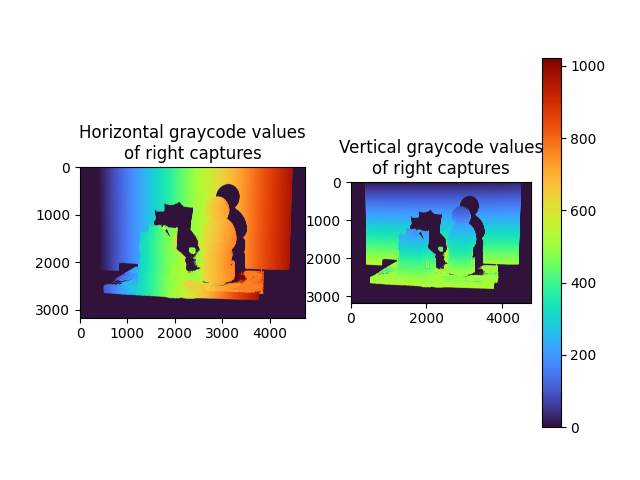
\includegraphics[height=50mm, keepaspectratio]{report_images/1_gray_codes/colormapped.png}
    \end{subfigure}
    \hfill
    \begin{subfigure}[b]{0.45\linewidth}
        \centering
        \includegraphics[height=50mm, keepaspectratio]{report_images/1_gray_codes/false_color.jpg}
    \end{subfigure}
    \caption{Gray code visualization using colormaps and false coloring with masking applied}
    \label{fig:graycodes_visualised}
\end{figure}

These visualizations already convey some sense of depth, as the Gray code values are spatially distorted due to the camera's perspective. To capture full 3D geometry, the structured light method is applied from two camera angles. Because the same pattern is projected from a fixed projector, pixels with matching Gray code values in both views correspond to the same physical point in the scene. This creates a dense set of correspondences, allowing for pixel-wise matching—unlike sparse feature-based methods—enabling point cloud reconstruction or computation of transformation matrices.

\section{Calibration}

To reconstruct a point cloud from matched Gray code values, camera calibration is essential, specifically the determination of the camera’s projection matrix. This is achieved using checkerboard calibration—a standard technique in computer vision to estimate intrinsic parameters.

Multiple images of a known checkerboard pattern are captured. The algorithm detects the checkerboard in each image and uses these detections to compute the calibration matrix. The calibration’s effectiveness is validated by undistorting the images.

OpenCV's \texttt{findChessboardCorners} function, refined by \texttt{cornerSubPix}, is used to detect corner points in the images. These 2D corners are mapped to a known 3D grid, assuming each square has a known size and lies on a flat plane. If a sufficient number of valid detections are found, \texttt{cv2.calibrateCamera} estimates the camera matrix and distortion coefficients. Distortion is then corrected using \texttt{cv2.getOptimalNewCameraMatrix} and \texttt{cv2.undistort}. Figure~\ref{fig:call} illustrates the calibration process.

\begin{figure}[H]
    \centering
    \begin{subfigure}[b]{0.45\linewidth}
        \centering
        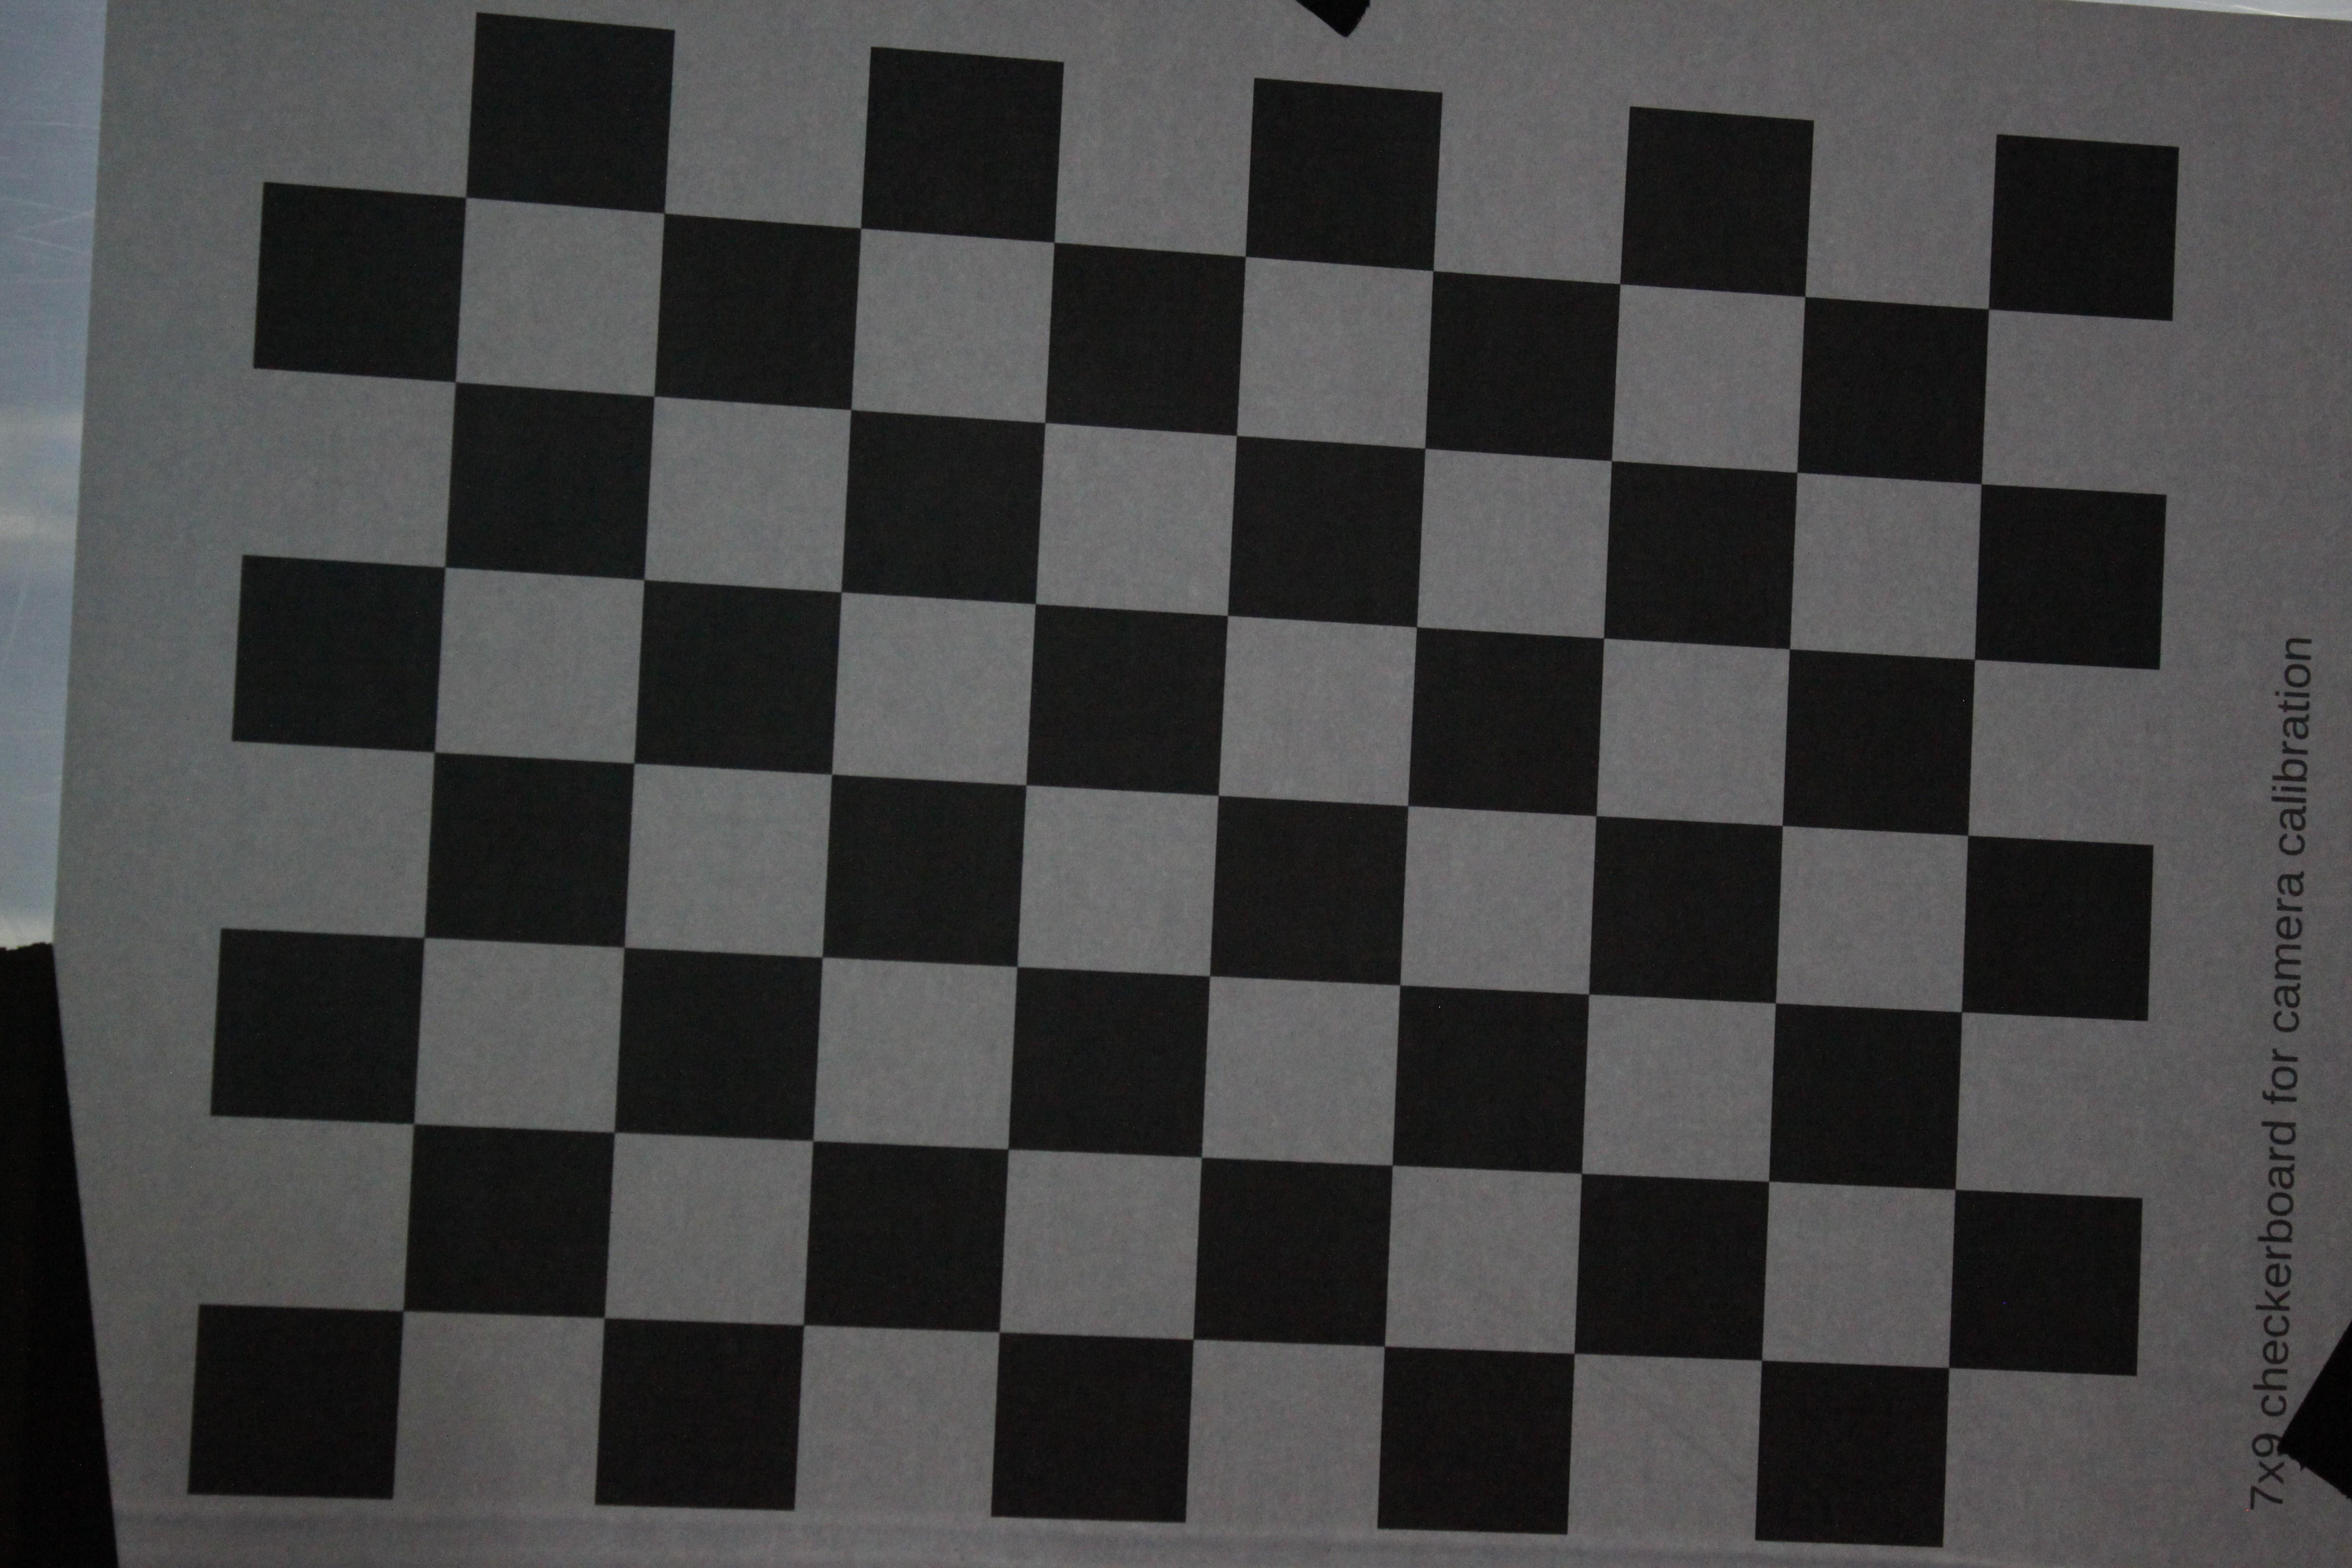
\includegraphics[height=50mm, keepaspectratio]{report_images/2Calibration/raw.jpg}
        \caption{Raw image}
    \end{subfigure}
    \hfill
    \begin{subfigure}[b]{0.45\linewidth}
        \centering
        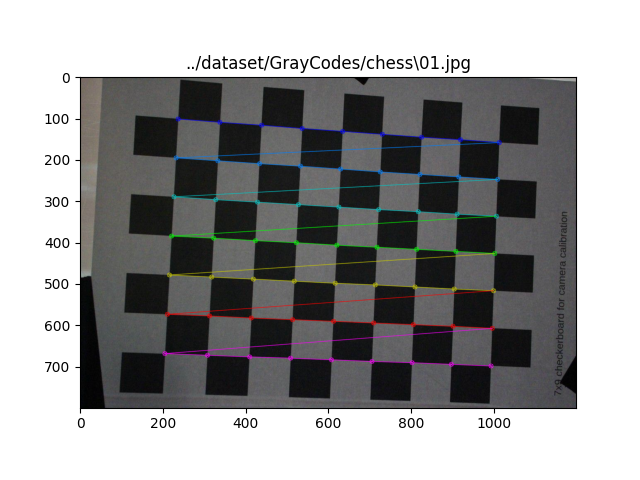
\includegraphics[height=50mm, keepaspectratio]{report_images/2Calibration/corners.png}
        \caption{Detected checkerboard corners}
    \end{subfigure}
    \hfill
    \begin{subfigure}[b]{0.45\linewidth}
        \centering
        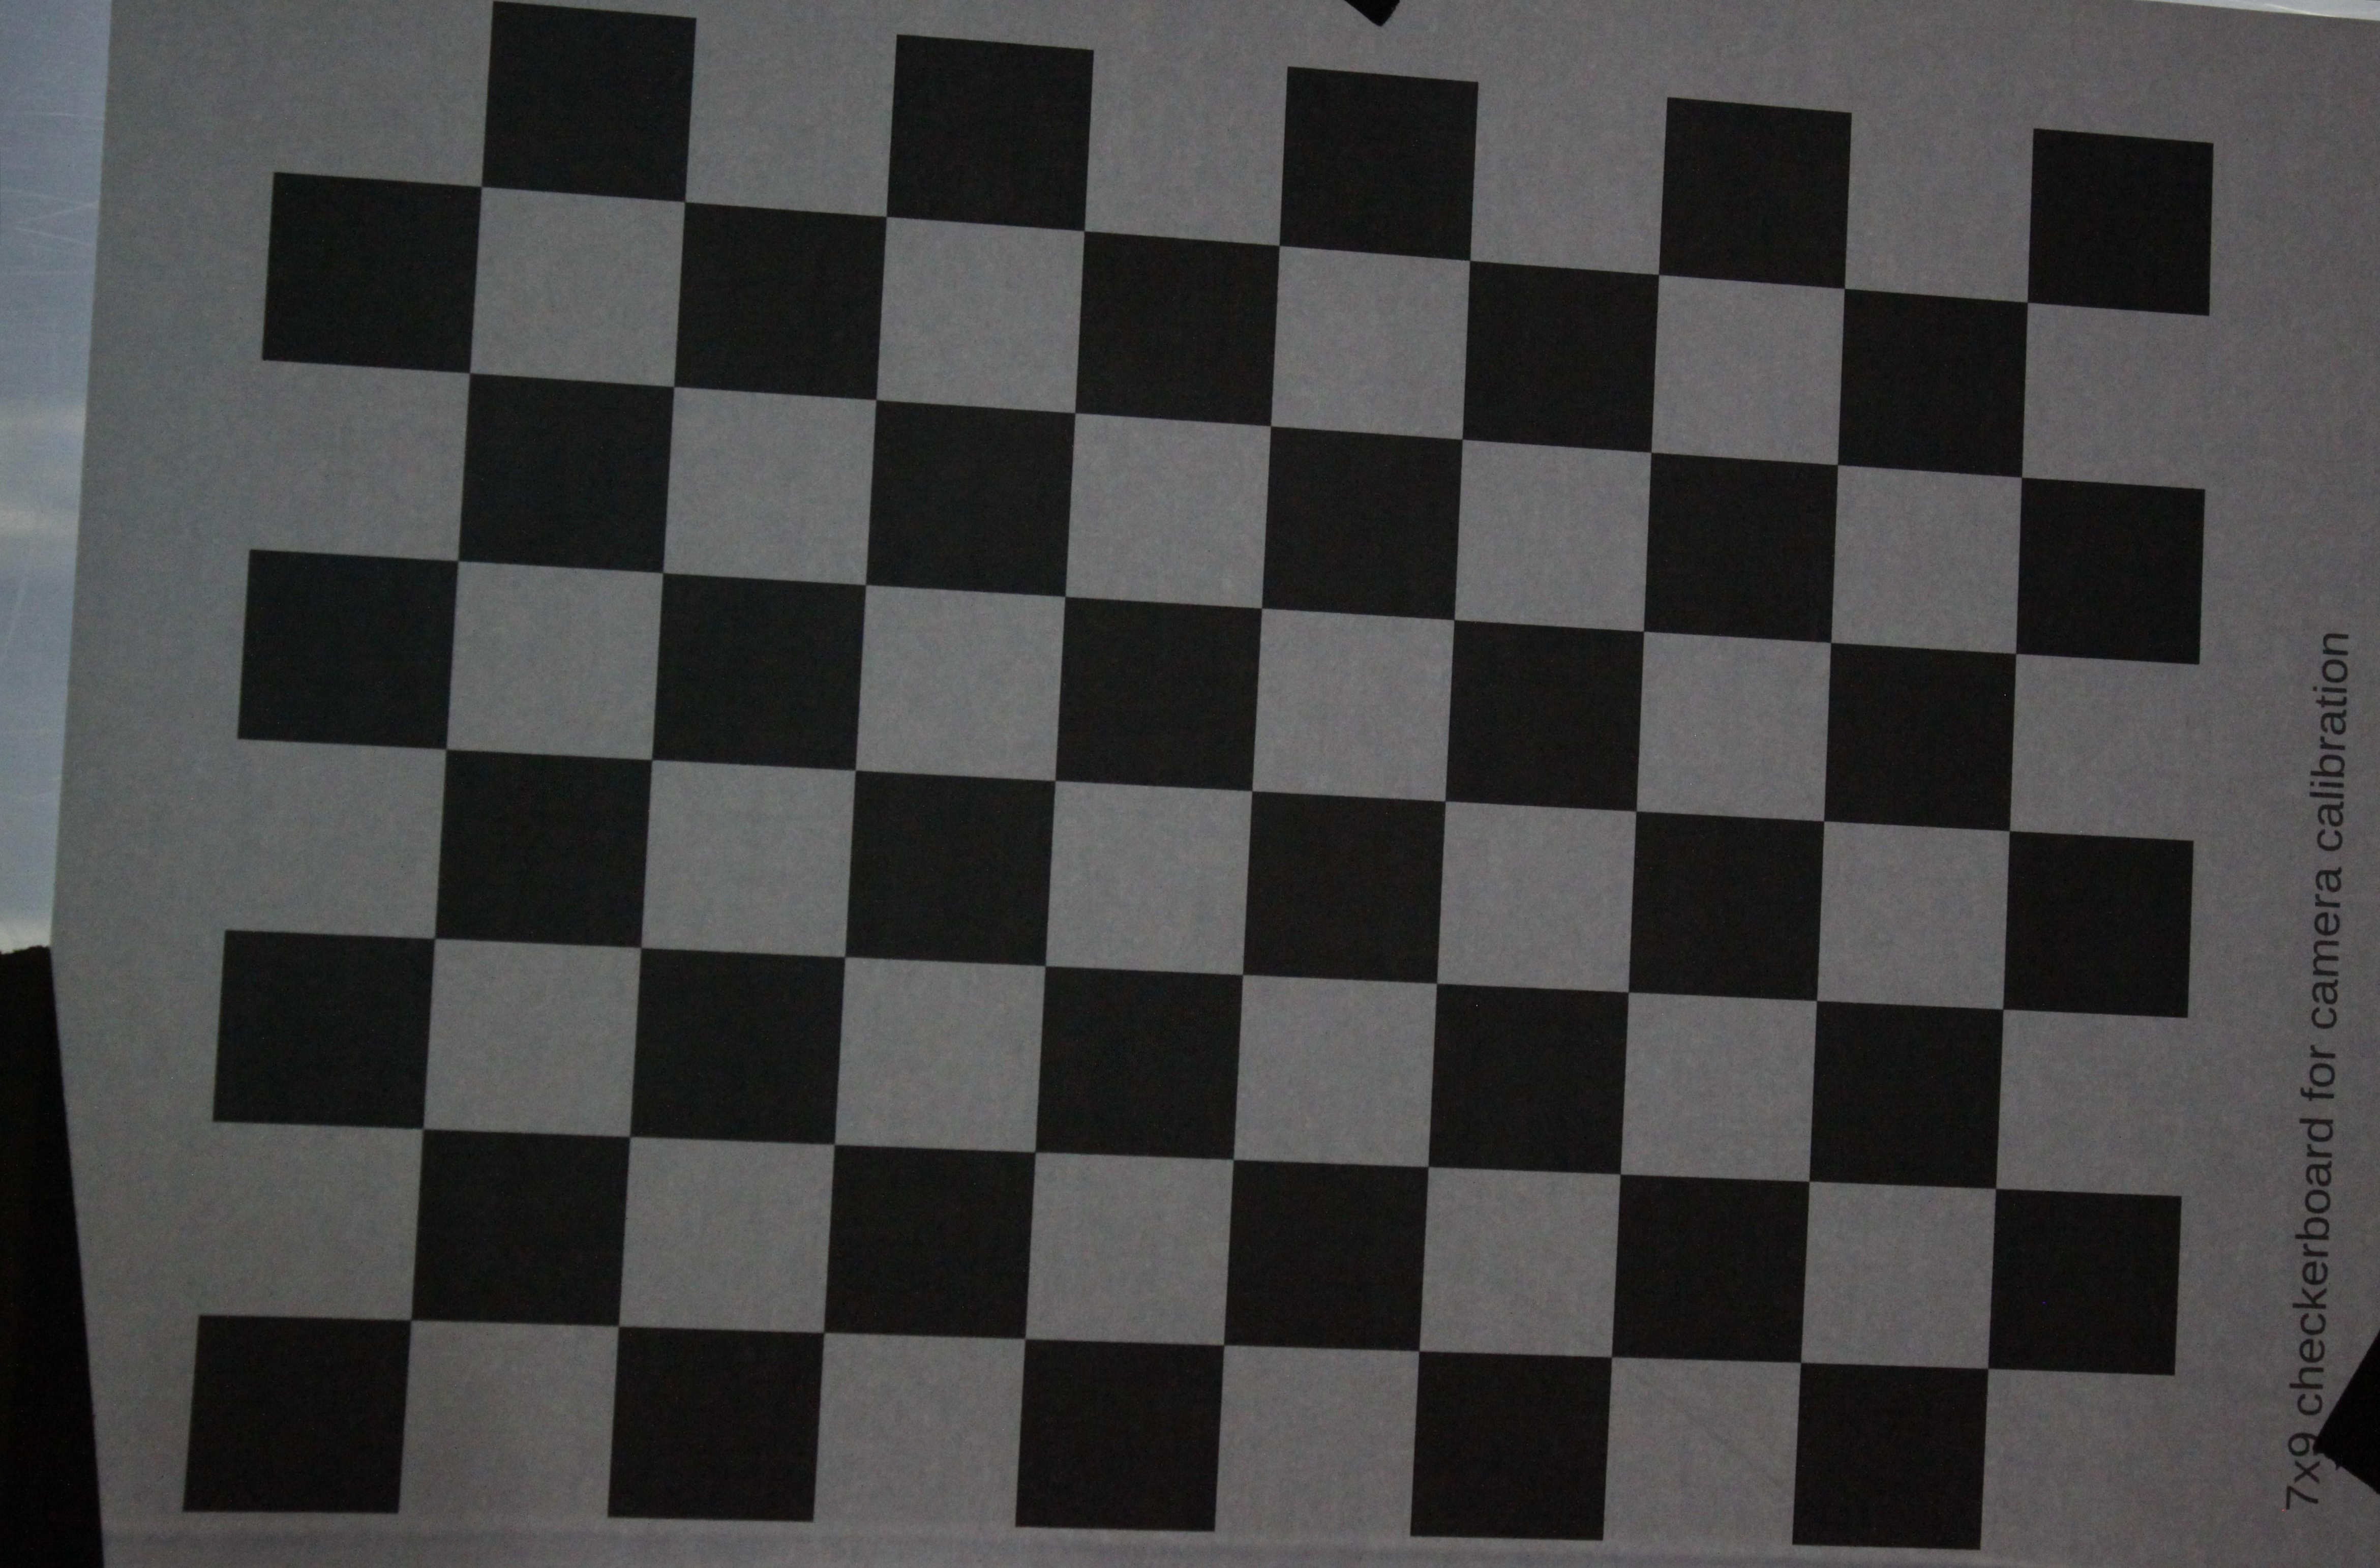
\includegraphics[height=50mm, keepaspectratio]{report_images/2Calibration/undistorted.jpg}
        \caption{Undistorted image}
    \end{subfigure}
    \caption{Camera calibration and distortion correction using checkerboard detection}
    \label{fig:call}
\end{figure}

\section{Point Cloud Reconstruction}

Given the Gray code maps from both the left and right camera views and the corresponding calibration matrices, a 3D point cloud can be reconstructed.

Stereo matching is necessary to compute depth. This requires the projection matrices and a dense set of matching points between the two images. Due to the unique spatial coding of Gray codes, these maps serve as a reliable basis for finding correspondences.

The matching algorithm iterates over the pixels in one Gray code map, storing each pixel’s coordinates using its Gray code value as a key in a dictionary. The same is done for the second map. Matches are found by looking up corresponding keys in both dictionaries. Only reliable pixels, as determined by the mask, are used. This results in a dense array of matched pixel coordinates. Figure~\ref{fig:match} shows a random sample of these matches.

\begin{figure}[H]
    \centering
    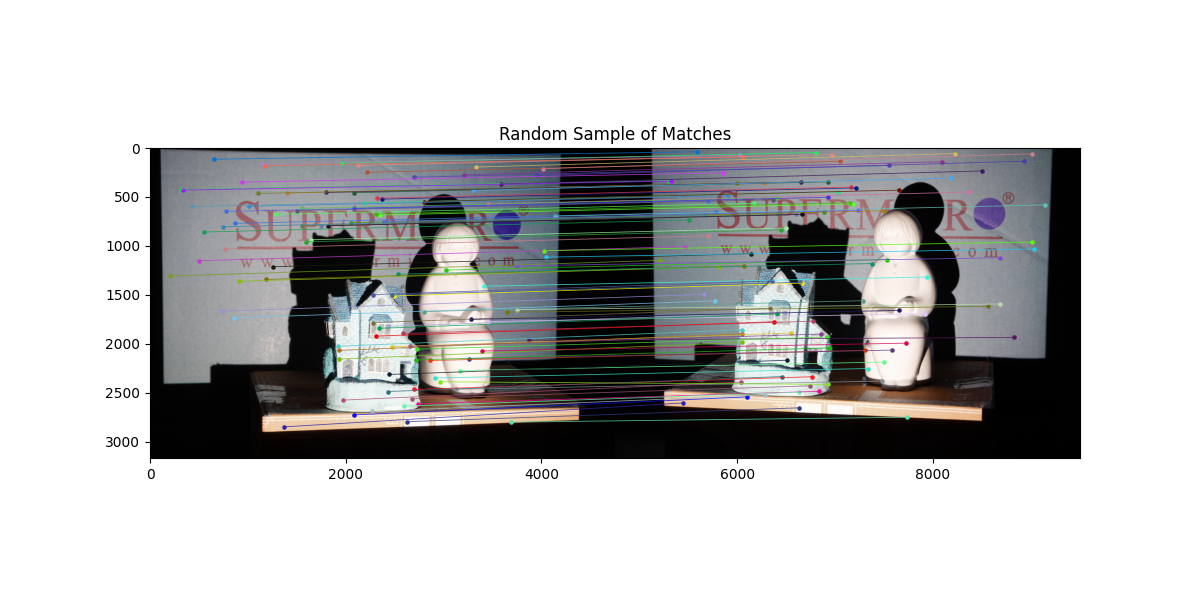
\includegraphics[height=80mm, keepaspectratio]{report_images/3_point_cloud/plotted_matches.png}
    \caption{Random sample of correspondences between left and right views}
    \label{fig:match}
\end{figure}

To compute the relative camera poses, \texttt{cv2.findEssentialMat} is used with the matched points to estimate the essential matrix, followed by \texttt{cv2.recoverPose} to extract the rotation and translation of the right view relative to the left. RANSAC is used to minimize the effect of outliers, which can be prevalent in dense match sets.

Projection matrices are then built using the known intrinsics and the recovered camera poses. The left camera uses an identity transformation, while the right uses the recovered rotation and translation. Using \texttt{cv2.triangulatePoints}, 3D coordinates are computed from the matched 2D points, producing a dense point cloud. Figure~\ref{fig:cloud} visualizes the result, with point colors sampled from the left image for realism.

\begin{figure}[H]
    \centering
    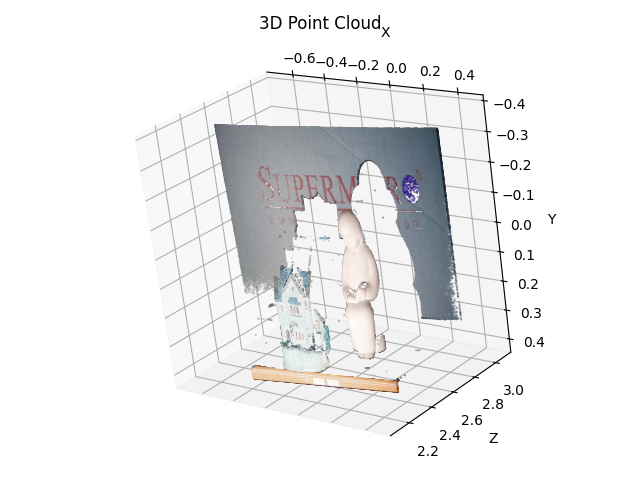
\includegraphics[height=100mm, keepaspectratio]{report_images/3_point_cloud/point_cloud.png}
    \caption{Reconstructed 3D point cloud of the scene}
    \label{fig:cloud}
\end{figure}

\end{document}
